\chapter{METODE PENELITIAN}
\label{BAB3:Metode}

Untuk menyelesaikan permasalahan yang dirumuskan, penelitian ini mengembangkan sistem \textit{chatbot} dengan arsitektur \textit{Unified RAG} yang mengintegrasikan metode konvensional dengan \textit{version-aware}. Metodologi penelitian dirancang untuk menangani dokumen yang memiliki riwayat perubahan (versi) secara kronologis.

\section{Desain Arsitektur Sistem}
Sistem dibangun berdasarkan arsitektur yang memisahkan antara komponen standar RAG dengan komponen logika versi. Gambaran umum arsitektur sistem dapat dilihat pada Gambar \ref{fig:rag_architecture}.
\begin{figure}[h]
    \centering
    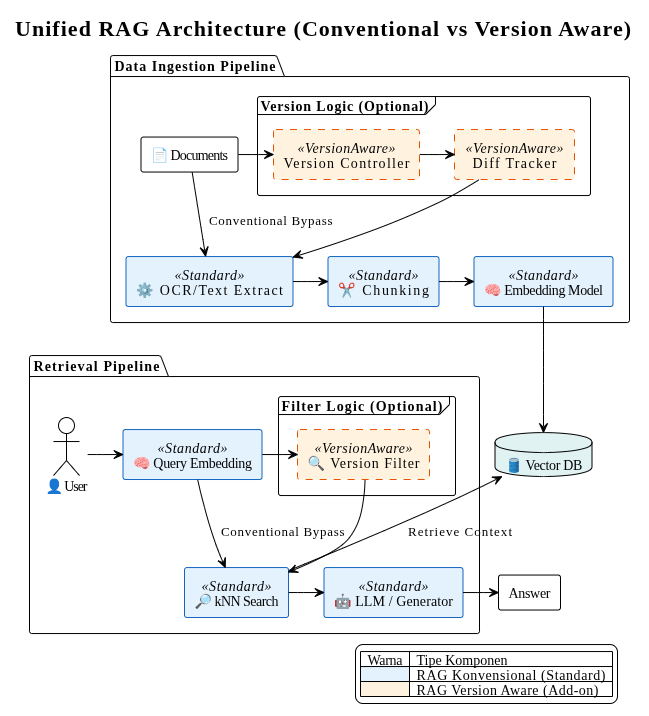
\includegraphics[width=0.7\textwidth]{BAB-3/rev-RAG-diagram.png}
    \caption{Arsitektur Unified RAG (Conventional vs Version Aware)}
    \label{fig:rag_architecture}
\end{figure}

Seperti yang ditunjukkan pada Gambar \ref{fig:rag_architecture}, arsitektur ini terdiri dari dua jalur utama (\textit{pipeline}):
\begin{enumerate}
    \item \textbf{\textit{Data Ingestion Pipeline}}: Bertanggung jawab untuk memproses dokumen mentah menjadi representasi vektor yang tersimpan dalam basis data.
    \item \textbf{\textit{Retrieval Pipeline}}: Bertanggung jawab untuk menangani pertanyaan pengguna, melakukan pencarian relevansi, dan menghasilkan jawaban.
\end{enumerate}

Komponen berwarna biru merepresentasikan proses RAG standar (\textit{Standard Component}), sedangkan komponen berwarna oranye dengan garis putus-putus merepresentasikan logika tambahan (\textit{Add-on Logic}) untuk menangani kapabilitas \textit{version-aware}.

\section{\textit{Data Ingestion Pipeline}}
Tahap ini digambarkan pada bagian atas Gambar \ref{fig:rag_architecture}. Proses ini bertujuan mengubah dokumen tidak terstruktur menjadi format yang dapat dipahami oleh mesin dengan menyertakan konteks versi.

\begin{enumerate}
    \item \textbf{\textit{Version Logic (Controller)}} \\
    Sebelum dokumen diproses secara fisik, \textit{Version Controller} mengidentifikasi metadata dokumen seperti Nomor Dokumen, Tag Versi (misalnya v1, v2), dan \textit{Timestamp}. Pada implementasi kode, logika ini memastikan setiap dokumen yang masuk ditandai dengan ID unik dan waktu unggah untuk membedakan antara dokumen lama dan dokumen terbaru.
    
    \item \textbf{\textit{OCR/Text Extract}} \\
    Dokumen PDF diproses menggunakan pustaka \textit{pdfplumber} dengan mode \textit{layout-aware} untuk mempertahankan struktur spasial teks. Jika dokumen berupa citra, sistem menggunakan \textit{pytesseract} (OCR) untuk mengekstraksi karakter visual menjadi teks digital.
    
    \item \textbf{\textit{Chunking}} \\
    Penelitian ini menerapkan metode \textit{Line-Aware Chunking}. Berbeda dengan pemotongan karakter statis, metode ini membagi teks berdasarkan baris logis yang telah dibersihkan dari karakter sampah (\textit{noise}). Setiap \textit{chunk} kemudian diasosiasikan dengan metadata versi yang telah disiapkan sebelumnya.
    
    \item \textbf{\textit{Embedding Model}} \\
    Teks yang telah terbagi dikonversi menjadi vektor numerik menggunakan model \textit{intfloat/multilingual-e5-base}. Model ini dipilih karena kemampuannya yang optimal dalam menangani teks multibahasa.
    
    \item \textbf{\textit{Vector DB}} \\
    Vektor dan metadata disimpan ke dalam \textit{ChromaDB}. Basis data ini bertindak sebagai jembatan penyimpanan antara proses \textit{ingestion} dan \textit{retrieval}.
\end{enumerate}

\section{\textit{Retrieval Pipeline}}
Tahap ini digambarkan pada bagian bawah Gambar \ref{fig:rag_architecture}, yang menjelaskan bagaimana sistem merespons masukan pengguna.

\begin{enumerate}
    \item \textbf{\textit{Query Embedding}} \\
    Pertanyaan pengguna dikonversi menjadi vektor menggunakan model yang sama dengan tahap \textit{ingestion}.
    
    \item \textbf{\textit{Version Filter (VersionAware Logic)}} \\
    Ini adalah komponen kunci yang membedakan penelitian ini dengan RAG konvensional. Sebelum atau sesudah pencarian vektor, sistem menerapkan filter logika:
    \begin{itemize}
        \item Jika pengguna meminta \textbf{versi spesifik} (misal: "Gunakan v1"), sistem memfilter metadata \texttt{version='v1'}.
        \item Jika pengguna meminta \textbf{versi terbaru} (\textit{Latest}), sistem melakukan pemfilteran pasca-pencarian (\textit{post-retrieval filtering}) untuk membandingkan \textit{timestamp} antar dokumen yang memiliki ID sama, dan hanya mengambil dokumen dengan waktu terkini.
    \end{itemize}
    
    \item \textbf{\textit{kNN Search}} \\
    Sistem melakukan pencarian \textit{k-Nearest Neighbors} (kNN) pada basis data vektor untuk menemukan potongan teks (\textit{chunks}) yang paling mirip secara semantik dengan pertanyaan pengguna, yang telah lolos dari tahapan \textit{Version Filter}.
    
    \item \textbf{\textit{LLM / Generator}} \\
    Konteks yang relevan disusun menjadi \textit{prompt} dan dikirim ke \textit{Large Language Model} (Ollama/Llama3). Model diperintahkan untuk menjawab hanya berdasarkan konteks yang ditemukan.
\end{enumerate}

\section{Evaluasi Model}
Untuk mengukur efektivitas arsitektur \textit{Version-Aware} ini dibandingkan dengan RAG Konvensional, dilakukan evaluasi menggunakan metrik RAGAS (\textit{Retrieval Augmented Generation Assessment}).

\begin{enumerate}
    \item \textbf{\textit{Context Precision}}: Mengukur apakah sistem berhasil mengambil versi dokumen yang tepat (misal: tidak mengambil dokumen v1 saat diminta v2).
    \item \textbf{\textit{Faithfulness}}: Mengukur seberapa akurat jawaban yang dihasilkan berdasarkan konteks versi yang diambil, tanpa halusinasi.
    \item \textbf{\textit{Answer Relevancy}}: Mengukur relevansi jawaban terhadap pertanyaan pengguna.
\end{enumerate}